\documentclass{article}
\usepackage{tikz}
\begin{document}
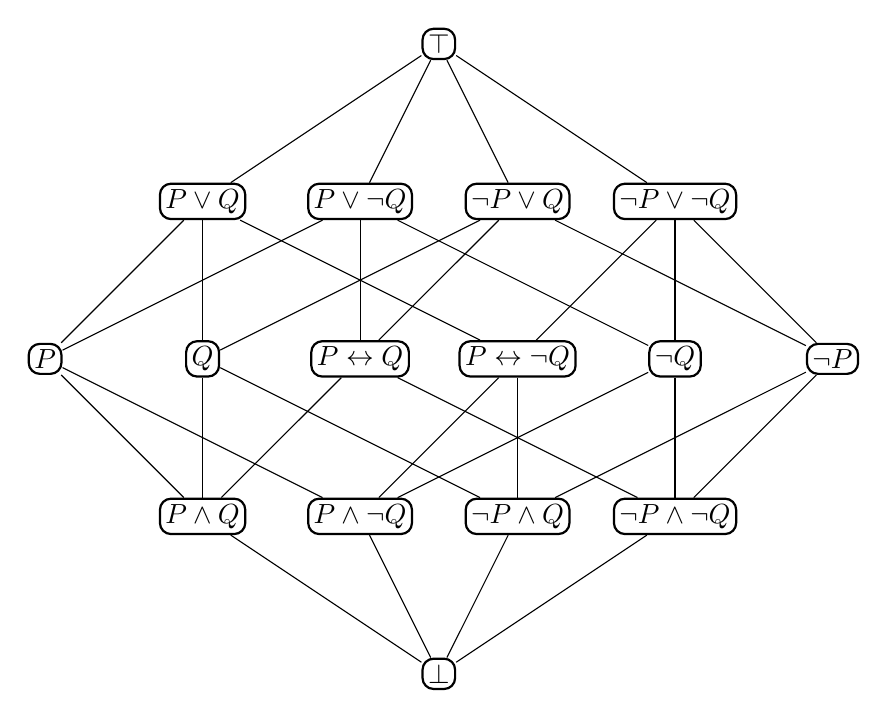
\begin{tikzpicture}[source/.style={draw,thick,rounded corners,inner sep=2pt}]
\node[source] (min) at (0,-1) {$\bot$};
\node[source] (A1) at (-3,1) {$P\wedge Q$};
\node[source] (A2) at (-1,1) {$P\wedge \neg Q$};
\node[source] (A3) at (1,1) {$\neg P\wedge Q$};
\node[source] (A4) at (3,1) {$\neg P\wedge \neg Q$};
\node[source] (B1) at (-5,3) {$P$};
\node[source] (B2) at (-3,3) {$Q$};
\node[source] (B3) at (-1,3) {$P\leftrightarrow Q$};
\node[source] (B4) at (1,3) {$P\leftrightarrow \neg Q$};
\node[source] (B7) at (3,3) {$\neg Q$};
\node[source] (B8) at (5,3) {$\neg P$};
\node[source] (C1) at (-3,5) {$P\vee Q$};
\node[source] (C2) at (-1,5) {$P\vee \neg Q$};
\node[source] (C3) at (1,5) {$\neg P\vee Q$};
\node[source] (C4) at (3,5) {$\neg P\vee \neg Q$};
\node[source] (max) at (0,7) {$\top$};
\draw (min) -- (A1);
\draw (min) -- (A2);
\draw (min) -- (A3);
\draw (min) -- (A4);
\draw (A1) -- (B1);
\draw (A1) -- (B3);
\draw (A1) -- (B2);
\draw (A2) -- (B1);
\draw (A2) -- (B4);
\draw (A2) -- (B7);
\draw (A3) -- (B2);
\draw (A3) -- (B4);
\draw (A3) -- (B8);
\draw (A4) -- (B3);
\draw (A4) -- (B8);
\draw (A4) -- (B7);
\draw (B1) -- (C1);
\draw (B1) -- (C2);
\draw (B2) -- (C1);
\draw (B2) -- (C3);
\draw (B3) -- (C2);
\draw (B3) -- (C3);
\draw (B4) -- (C1);
\draw (B4) -- (C4);
\draw (B7) -- (C2);
\draw (B7) -- (C4);
\draw (B8) -- (C3);
\draw (B8) -- (C4);
\draw (C1) -- (max);
\draw (C2) -- (max);
\draw (C3) -- (max);
\draw (C4) -- (max);
\end{tikzpicture}


\end{document}





%%% Local Variables:
%%% mode: latex
%%% TeX-master: t
%%% End:
